%# -*- coding: utf-8-unix -*-
%%==================================================
%% chapter_4.tex for SJTU Master Thesis
%%==================================================

\chapter{基于离线神经网络及PID控制的时钟伺服系统可行性研究}
在第\ref{chap:statistical_delay}章中,本人从链路传输延时的角度,通过深入分析实际工业环境下对链路传输延时的影响,通过对链路传输延时建立细致的数学模型,并从数学统计的角度对其中各个影响因素提出了有针对性的解决方案。

至此,我们已经能够利用上述算法综合获得稳定和精确的链路延时。但是,仅仅获取稳定精确的链路延时并不是时钟同步的终点。而且,在现实IEEE1588协议运行中,之所以同步精度难以达到亚微秒的同步精度,有很重要的因素是从时钟校正策略的选取。所谓时钟同步,最核心一环自然是从时钟根据计算数据对本地进行校正来实现同步,即时钟伺服系统。

常规我们在IEEE1588协议中采用的是PI控制策略,即利用PI控制器来对从时钟进行校正,而不是直接利用offset进行校正。这种做法能够一定程度提高从时钟的同步精度和稳定性,但它也存在如PI参数固定等缺陷而导致同步系统无法有效应对复杂多变的工业网络环境,这严重破坏了从时钟系统的鲁棒性和稳定性。因此,考虑到工业网络环境的复杂性和多变性,本文尝试从神经网络控制策略入手,以期待利用神经网络优秀的适应性来提高从时钟对复杂环境的鲁棒性和自适应性。

\section{时钟伺服系统研究}
对从时钟而言,如果想要实现与主时钟同步,就必须依靠前面提到的同步算法及所计算出来的链路时延值,从而对从时钟自身的相位和频率进行校正,以有效消除与主时钟之间的偏差。不过,由于当前的很多工业平台并非实时操作系统,所以一般而言都需要利用中断机制来触发从时钟进行校正。但是,在该中断过程中造成的从时钟漂移抖动会长期破坏同步精度,严重影响同步过程的实时性。

因此,为了提高从时钟校正过程的实时性和快速性,我们需要设计一套比较良好的时钟伺服系统来对从时钟进行校正。

\subsection{通用PTP时钟伺服系统介绍}

\begin{figure}[!hbp]
  \centering
  \begin{minipage}[b]{0.7\textwidth}
    \captionstyle{\centering}
    \centering
    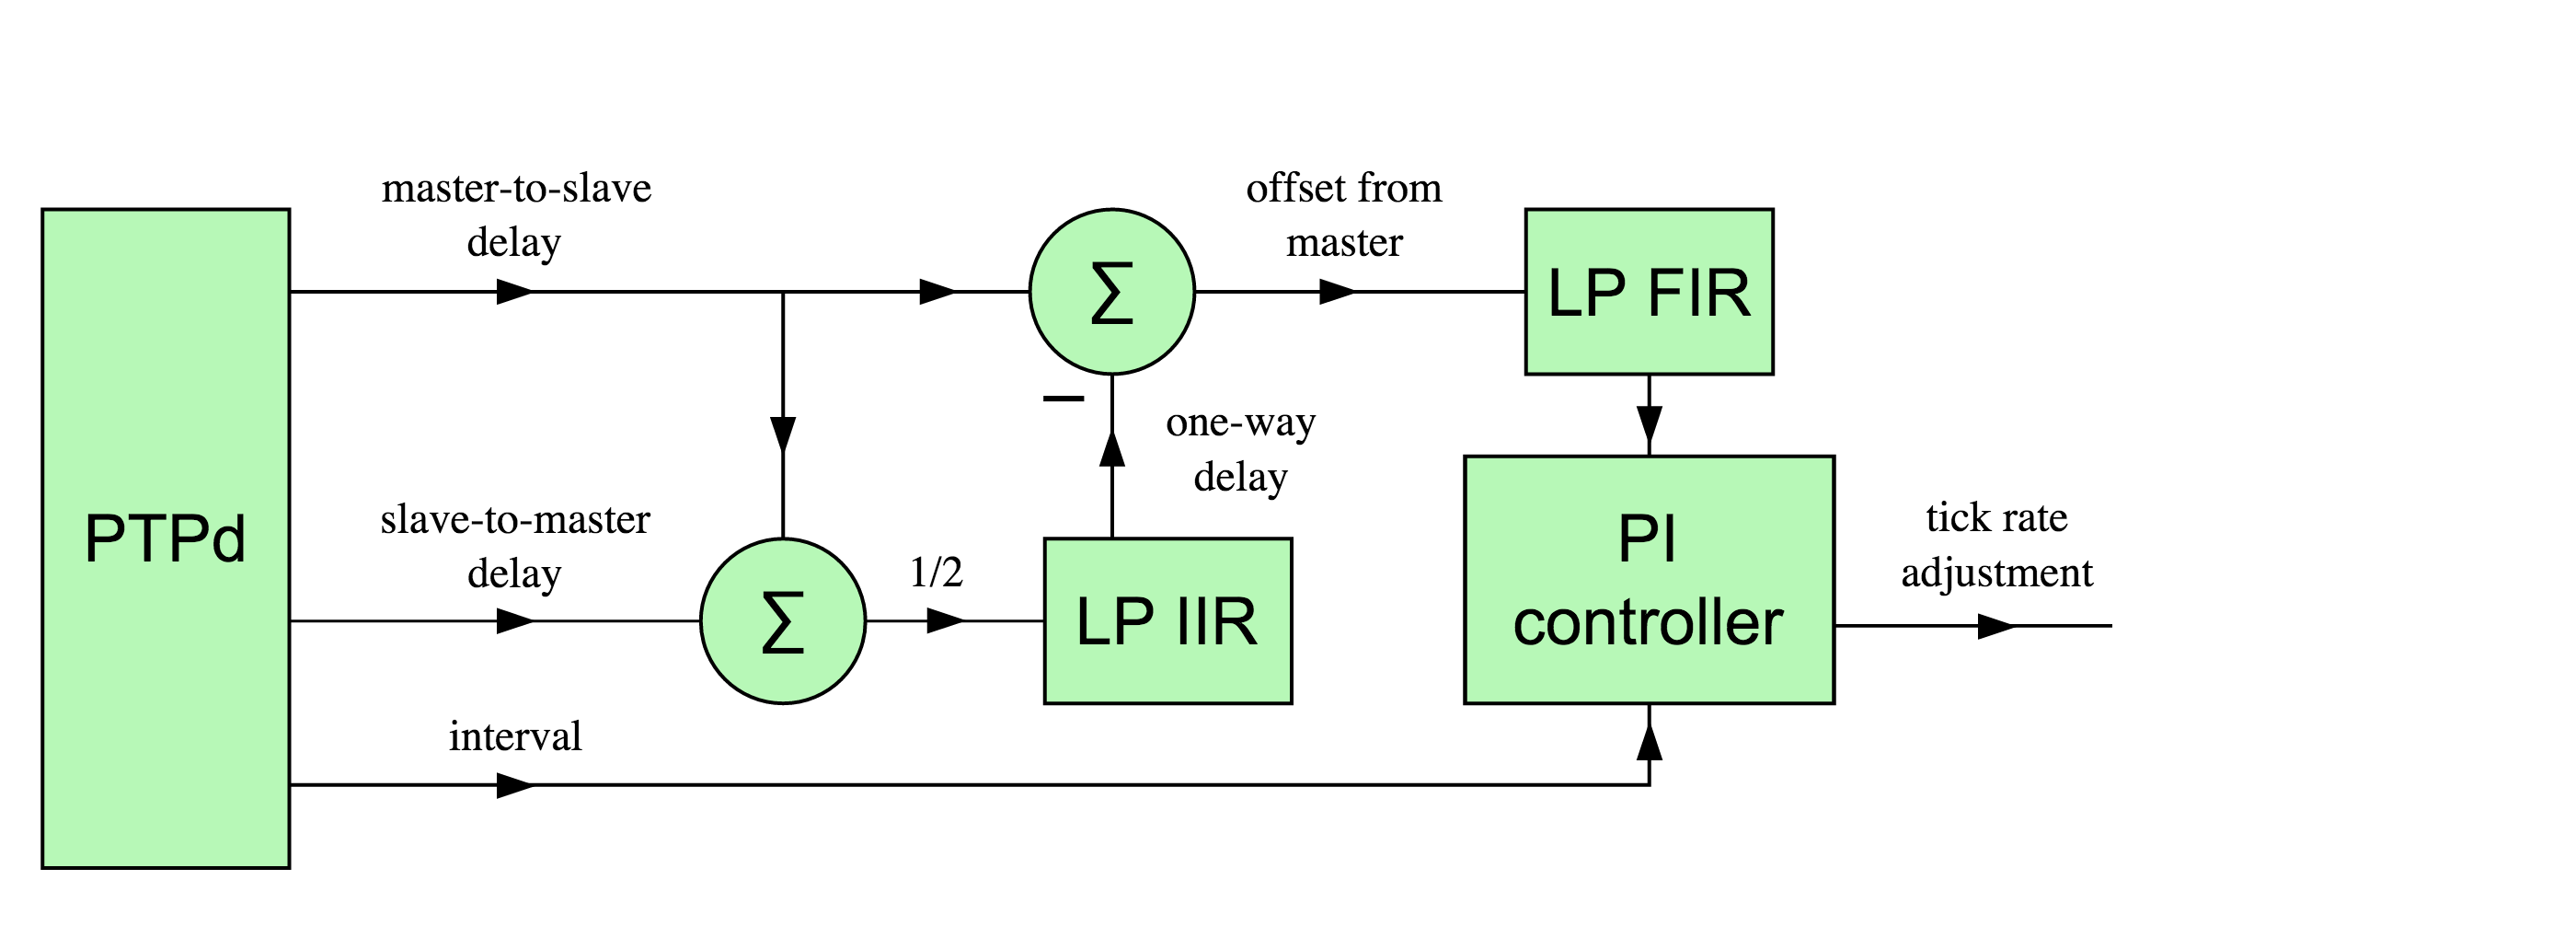
\includegraphics[width=11cm]{normal_clock_servo_system}
    \bicaption[fig:normal_clock_servo_system]{通用PTP时钟伺服系统}{通用PTP时钟伺服系统}{Fig}{The normal structure of general PTP clock servo system}
  \end{minipage}     
\end{figure}

一种常见的PTP时钟伺服系统如上图\ref{fig:normal_clock_servo_system}所示。从左到右表明了数据从PTP协议引擎逐渐流向从时钟。在该系统中,PTP协议引擎通过周期性获取主从偏差和从主偏差,将这两个偏差值通过均值滤波及低通滤波器获取到当前offset值。然后,将当前offset值与采样周期数据共同传递给PI控制器,由PI控制器来对从时钟进行校正以实现主从同步。该PI控制器由比例(P)和积分(I)两个环节共同构成,其中,比例环节可以用来消除主从时钟间的相位偏差,而积分项则可以用来消除系统的稳态误差,即消除主从时钟间的频率差\supercite{58}。

上述这样一套较为完整的时钟伺服系统可以较好的实现时钟同步,而且,由于传统的PI控制算法相对而言比较简单、鲁棒性良好且可靠性较高,所以传统的PI控制器在工业控制领域里应用十分广泛。

但是,传统的PI控制器也有其固有的弊病,那就是其比例积分参数的调整往往需要依靠经验来设定。对于处于复杂网络环境中的时钟同步系统而言,仅仅依靠经验来整定控制参数的PI控制器几乎无法应对任何形式的复杂多变的环境,尤其是同步系统中的网络环境中存在多种非线性、时变性等不确定性因素时,被控对象特性常常会随着时间发生变化。例如工业中充当从时钟的PTP设备,很容易会随着时间慢慢精度降低,并且长期受到工业干扰导致设备性能逐渐下降\supercite{59}。这些从时钟的变化都会导致传统的PI控制器在时钟伺服系统中无法达到良好的控制效果。

所以,为了使得时钟伺服系统能够适应工业网络环境变化,尤其是应对时变性非常强的网络传输环境,本人在下文从智能自适应控制的角度出发,结合同步系统特性进行深入分析,并且提出基于智能控制策略作为伺服系统中的控制环节,从而来弥补传统PI控制器无法适应复杂网络环境的缺陷。

\subsection{智能控制策略介绍}
随着被控对象及控制环境的越来越复杂,越来越多的智能控制策略依次出现,而且到现在为止已经被广泛地应用到了工业网络控制系统中。以网络控制系统中的时延不确定性为例,当前工业中陆续采用了多种智能控制方法来提高系统的鲁棒性和抗干扰性\supercite{19,20}。文献\parencite{21}中,作者通过对实际的Internet控制系统的时延数据分析,从而对控制系统建立了状态反馈模糊控制器;文献\parencite{22}采用了动态模糊控制器,对基于TCP/IP网络的远程伺服控制系统进行了研究;文献\parencite{23}中作者针对Ethernet提出了一种改进型神经元PID控制器,该控制器可以不依赖于网络时延精确数学模型。这些研究成果都表明对于复杂的网络环境,我们可以采用智能控制策略来进行自适应控制,而且能够取得良好的控制效果。

\section{基于神经网络的PID控制策略}
根据上节可以知道,由于传统PI控制器无法适应网络传输环境和被控对象的时变性,我们需要采用一种能够自动根据当前网络环境而调整的控制策略。本人在此选择神经网络及PI控制相结合,以此来实现时钟伺服系统中对从时钟的控制。下文会对该控制策略进行详细讲解。

\subsection{神经网络介绍与研究}
\subsubsection{神经网络特征}
神经网络\footnote{Neural Network}是一种由大量处理单元,也可以称为神经元,广泛连结而成的网络。通过对人类大脑工作机理的认识,并且把人脑的活动规律和组织结构作为背景,从而来反映人脑的一些基本特征\supercite{61}。或者可以认为,所谓神经网络,可以看作是对人脑的某种抽象和模仿。而从本质上来讲,神经网络也是一个数学模型,通过背后的计算机等电子器件来对人的智能进行模拟,其核心支持来源于神经科学、统计学、数学、计算机科学等多种学科。另外我们也知道,神经网络不单纯是高度非线性动力学系统,而且还是自适应系统。我们可以利用神经网络模型来描述认知决策和控制等智能行为。

除此之外,我们知道神经网络具备存储和应用经验知识的重要特点,与人脑相比,它具备以下两个相似之处:
\begin{itemize}[noitemsep,topsep=0pt,parsep=0pt,partopsep=0pt]
	\item 可以通过学习来从外部环境中获取知识,即使在不断变化的复杂环境下,它仍然能够通过不断的学习来适应这种环境的变化。
	\item 内部神经元具有存储知识的能力,只要神经网络对某种环境进行了学习,那么所积累下来的经验就会一直存在于神经网络内部,并且会在未来的继续学习中不断调整和改良。
\end{itemize}

\subsubsection{神经网络基本原理及构造}
神经网络作为模拟人的思维方式,它内部的单元多数都使用结构较为简单的神经元模型,然后通过对内部神经元之间的权值进行修正从而来实现对多维数据的非线性处理\supercite{61}。

\begin{figure}[!hbp]
  \centering
  \begin{minipage}[b]{0.6\textwidth}
    \captionstyle{\centering}
    \centering
    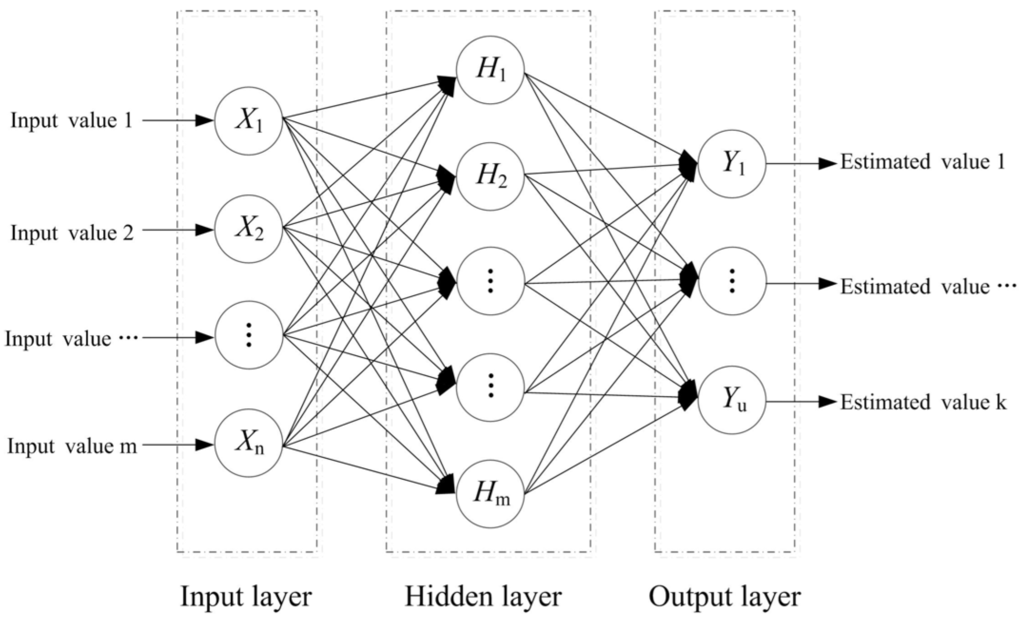
\includegraphics[width=10cm]{neural_network}
    \bicaption[fig:neural_network]{神经网络结构图}{神经网络结构图}{Fig}{The structure of neural network}
  \end{minipage}     
\end{figure}

根据图\ref{fig:neural_network}可以看到神经网络的整体结构,在一套完整的神经网络结构中,一般会包含多个不同的网络层单元,即下列几个网络层:
\begin{itemize}[noitemsep,topsep=0pt,parsep=0pt,partopsep=0pt]
	\item 输入层(Input Layer):这一层的输入节点主要接收外部数据的特征变量。对于这些特征变量的选取,必须能够准确地描述外界事物,依据选择对象的特征来选择有意义的原始特征变量,这也称为特征空间。所以说,这一层中会有大量神经元接受外界复杂的非线性输入信息。
	\item 隐含层(Hidden Layer):这一层是中间层,即位于输入层与输出层之间的一层,包含众多神经元和链接。事实是隐含层可以有多层,但习惯上我们只会用一层。这一层的节点数目不定,但数目越多的话,对应的网络非线性越显著,使得神经网络的强健性更为明显\footnote{强健性即控制系统在一定结构、大小等的参数摄动下,维持某些性能的特性。}。一般而言可以选输入节点数1.2至1.5倍的节点。
	\item 输出层(Output Layer):这一层是神经网络经过计算后将计算值对外输出的一层。所有原始数据在神经元节点中进行传输、分析,最终形成输出结果,我们把输出的信息结果数据称为输出向量。
\end{itemize}

\subsubsection{神经网络训练过程}
以“聚类”为例子,为了将具备相同属性的对象归为同一类,首先,神经网络方法会将每个簇描述为一个标本,然后,神经网络会根据计算得出的特定的距离度量,把新的对象依据距离度量值分配给与该标本最相似的簇。最终,对于一个簇而言,所有的对象的属性都可以根据该簇标本的属性来进行预测\supercite{67}。在神经网络内部的处理单元中,我们会采用相关的数学函数来对数据进行处理。而且,此处可以将多个处理单元连接称为系统,即可以创建一个智能模型。

在神经网络开始训练之前,我们必须把需要将输入单元、处理单元和输出单元进行连接。训练过程中,我们要对输入元和输出元之间的连接权值进行修正。具体的修改方式要依据其对某一结果的重要程度来进行调解。在这里,我们必须选择某种特定的学习规则来对权值进行调节。

最终,我们通过历史样本数据来对神经网络进行反复的训练,同时对各个处理单元之间的权值不断修改。当最终输出的结果与已知结果吻合度达到足够高时,我们就可以认为训练完成并停止训练。\supercite{67}。

\subsection{神经网络与时钟伺服系统的关联性研究}
之所以本文会采取神经网络作为时钟伺服的控制学习策略,主要基于以下几点考虑:
\begin{itemize}[noitemsep,topsep=0pt,parsep=0pt,partopsep=0pt]
	\item 神经网络是高度非线性动力学系统,又是自适应自组织系统,而我们的时钟同步系统所在的工业网络环境也是非常复杂且时变的,所以,我们需要一个学习策略能够根据外界网络环境的变化来调节自身,具备良好自适应性\supercite{64}。因此,神经网络是一个很好的选择。
	\item 神经网络具备学习功能,即通过学习大量的样本数据来获取输入输出之间的函数关系,这对于数学模型复杂或难以建立的系统具备良好的适应性,而我们的从时钟系统便由于工业现场的多变性而难以建立准确的数学模型。因此,神经网络能够发挥样本数据的优势来解决。
	\item 神经网络是一种数据非线性映射工具,相对于传统统计的数学方法而言,不仅不会产生冲突,而且可以互相补充\supercite{68}。由上文介绍知道,本文中采用了多种数学统计方法,也积累了很多样本数据,因此,数学统计策略与神经网络模型可以良好的结合在一起。
\end{itemize}

因此,由于神经网络高度的自学习能力,非常适合模拟复杂的非线性系统。根据神经网络理论中的Kolmogorov连续性定理,给定任一连续函数
\begin{align}
f:[0,1] \quad n \rightarrow Rm
\end{align}
f,我们都可以用一个三层前馈神经网络来精确地实现,从数学上保证了神经网络用语时间序列预测的可行性。而且,本文中采用了多种数学统计方法,积累了很多的样本数据,而神经网络作为数据非线性映射工具,可以和前面所提的数学统计方法得到非常良好的结合。

\subsection{BP神经网络原理}
1985年,Rumelhart等人提出的一种神经网络算法,即BP反向传播算法\footnote{back propagation},这是一种多层前馈网络所使用的有监督的学习过程。这个算法主要利用给定的输入、输出样本来进行学习,并且可以利用网络实际输出与期望输出的误差来进行反馈调节偏差,通过反向传递该偏差值来进一步调整网络的连接权值,最终完成神经网络的训练过程。该BP误差反向传播学习算法一般而言会基于最小均方差准则,并结合使用梯度下降法来在误差曲面搜索误差函数的极小值,然后利用计算结果来调整连接权值,最终使得误差函数极小化\supercite{65}。具体有如下几个步骤:
\begin{enumerate}[noitemsep,topsep=0pt,parsep=0pt,partopsep=0pt]
	\item 输入样本,利用选定的激励函数来计算各结点输出值:
	 	\begin{align}
	 		O = f(\omega \cdot x)
	 	\end{align}
	 	在这个过程中,我们选择Sigmoid函数,该函数是一类在应用中最普遍的激励函数。在[0,1]区间上,我们可以按如下表示Sigmoid函数表达式及导数:\\
	 	原函数形式:
	 	\begin{align}
	 		f_{1}(x) = \frac{1}{(1 - exp(-\lambda x))}
	 	\end{align}
	 	导数形式:
		\begin{align}
	 		f_{1}'(x) = \lambda f_{1}(x)[1-f_{1}(x)]
	 	\end{align}
	 \item 使用以下的误差函数公式计算神经网络输出与期望之间的均方差:
	 	\begin{align}
	 		E(\omega) = 0.5\sum_{k\in Input Layer}(t_{k} - o_{k})^{2}
	 	\end{align}
	 	在上式中,样本的期望输出值表示为$t_{k}$,对于网络输出层的第k个结点的实际输出值为$o_{k}$,其中k为网络层输出节点。
	 \item 通过反向传播的计算方法,计算输出层中每个输出节点的误差项:
	 	\begin{align}
	 		\delta_{k} = o_{k}'(t_{k} - o_{k}) = o_{k}(1 - o_{k})(t_{k} - o_{k})
	 	\end{align}
	 \item 在隐含层中,我们对其中所有节点计算当前实际输出值的下对应的误差项:
	 	\begin{align}
	 		\delta_{h} = o_{h}'\sum_{k}\omega_{hk}\delta_{k} = o_{h}(1 - o_{h})\sum_{k}\omega_{hk}\delta_{k}
	 	\end{align}
	 	其中,我们用k来表示输出节点,用h来表示隐含层节点。
	\item 然后我们要计算每个连接权值的修正值,这里用$\eta$ 来表示学习率,$\eta$ 越小,则训练收敛时更稳定,但所消耗的收敛时间会更长;
	相反,$\eta$ 越大,则收敛速度越快,但是,这也会使得系统稳定性变差。
	 	\begin{align}
	 		\Delta \omega_{ji} = \eta \delta_{j} x_{ji}
	 	\end{align}
	 \item 依据上一步的计算结果,可以对各连接权的权值进行调整,然后继续从第一步开始处理。
	 	\begin{align}
	 		\omega_{ji} = \omega_{ji} + \Delta\omega_{ji}
	 	\end{align}
	 	当响应单元的输出值接近0或1时,Sigmoid导数的值将接近于0、1。
\end{enumerate}

\subsection{BP神经网络的改进}
在对称型Sigmoid激励函数的神经网络中,会存在所谓的饱和区域,当响应单元输出值接近-1或者1时也存在这样的现象。而我们知道Sigmoid导数值用于反馈误差中的修正值计算,所以当Sigmoid函数进入饱和区域时,我们利用权值修正公式计算出来的权值修正量就会变得非常小,从而导致网络的训练陷入饱和状态,这种状态会大大降低网络的学习效率。因此,为了修正BP神经网络中的这些固有缺陷,一般会从一下两种角度来进行改进:一种是基于标准数值最优化的改进方法,如LM算法\footnote{Levenberg-Marquardt}、拟牛顿算法或者共轭梯度算法;另一种是基于标准梯度下降的改进方法,如弹性BP算法、自适应学习速率法和增加动量项的BP算法等\supercite{65}。下面主要对增加动量法作简单介绍。

我们知道,标准BP算法在本质上,是一种最速下降静态寻优算法,也就是说,当它在进行权值$\omega(k)$ 修正时,它会完全按照当前负梯度方式来修正,而不会把以前经验考虑进来,也就是过去时刻的梯度方向。这种行为很有可能是的学习过程收敛得非常缓慢,甚至可能会发生振荡。因此,对于这个缺陷,我们采取将上次权值调整值的部分累加到当前误差计算所得权值调整值上来的到当前实际权值调整量。从而使BP神经网络在进行权值修正时,不仅需要考虑误差在梯度上的作用,而且还需要对其对于误差曲面变化趋势的影响考虑进来。即:
\begin{align}
	\omega(k+1) = \omega(k) + \eta[(1-a)D(k) + aD(k-1)]
\end{align}
其中,$\omega(k)$表示当前时刻的权值向量,D(k)表示负梯度方向k训练阶段的值为学习率,最重要的是在这个学习过程中引入了a系数,我们称之为动量因子,
\begin{align}
	a \in [0, 1]
\end{align}
当神经网络在附加动量因子的方法下进行训练时,a参数不仅能够减小学习过程的振荡幅度,还能够降低网络对于误差曲面局部细节的敏感度,从而把网络陷入局部极小的状态进行抑制,提高系统使其具有更好的收敛性。

\section{基于BP神经网络的PID控制策略实现}
由上文可知,对于时钟同步系统而言,由于工业网络环境复杂且时刻变化,简单的PI控制完全无法应对多变的环境,也不具备任何自适应性。所以,仅仅采用简单的PI控制无法使的从时钟系统能够达到很好的稳定性和收敛性,甚至可能由于网络环境的不断变化而发生振荡甚至难以稳定。因此,一种能够控制非线性且时变的对象的控制策略对于工业环境下时钟同步系统而言至关重要。

在上一小节中,本人通过对神经网络基础原理及相关理论进行了较为深入的研究。可以看出,神经网络算法不仅具备良好的学习功能,这能帮助从时钟在复杂的网络环境下不断对自身进行调整以达到良好的同步效果,而且,该算法作为数据非线性映射工具,还能与传统统计方法相互补充,而本人在前面已经采取了多种统计算法,所以,在从时钟端会累积很多样本数据,这些样本的存在正好使的神经网络算法发挥更大的作用\supercite{63}。

为了将神经网络算法应用于时钟伺服系统中,我们可以将神经网络与PID控制系统相结合,通过外界输入样本对神经网络进行训练,然后让神经网络对外输出PID控制系统所需要的三种控制参数$K_{i}$、$K_{p}$、$K_{d}$。可以参考下图的结构设计:

\begin{figure}[!hbp]
  \centering
  \begin{minipage}[b]{0.6\textwidth}
    \captionstyle{\centering}
    \centering
    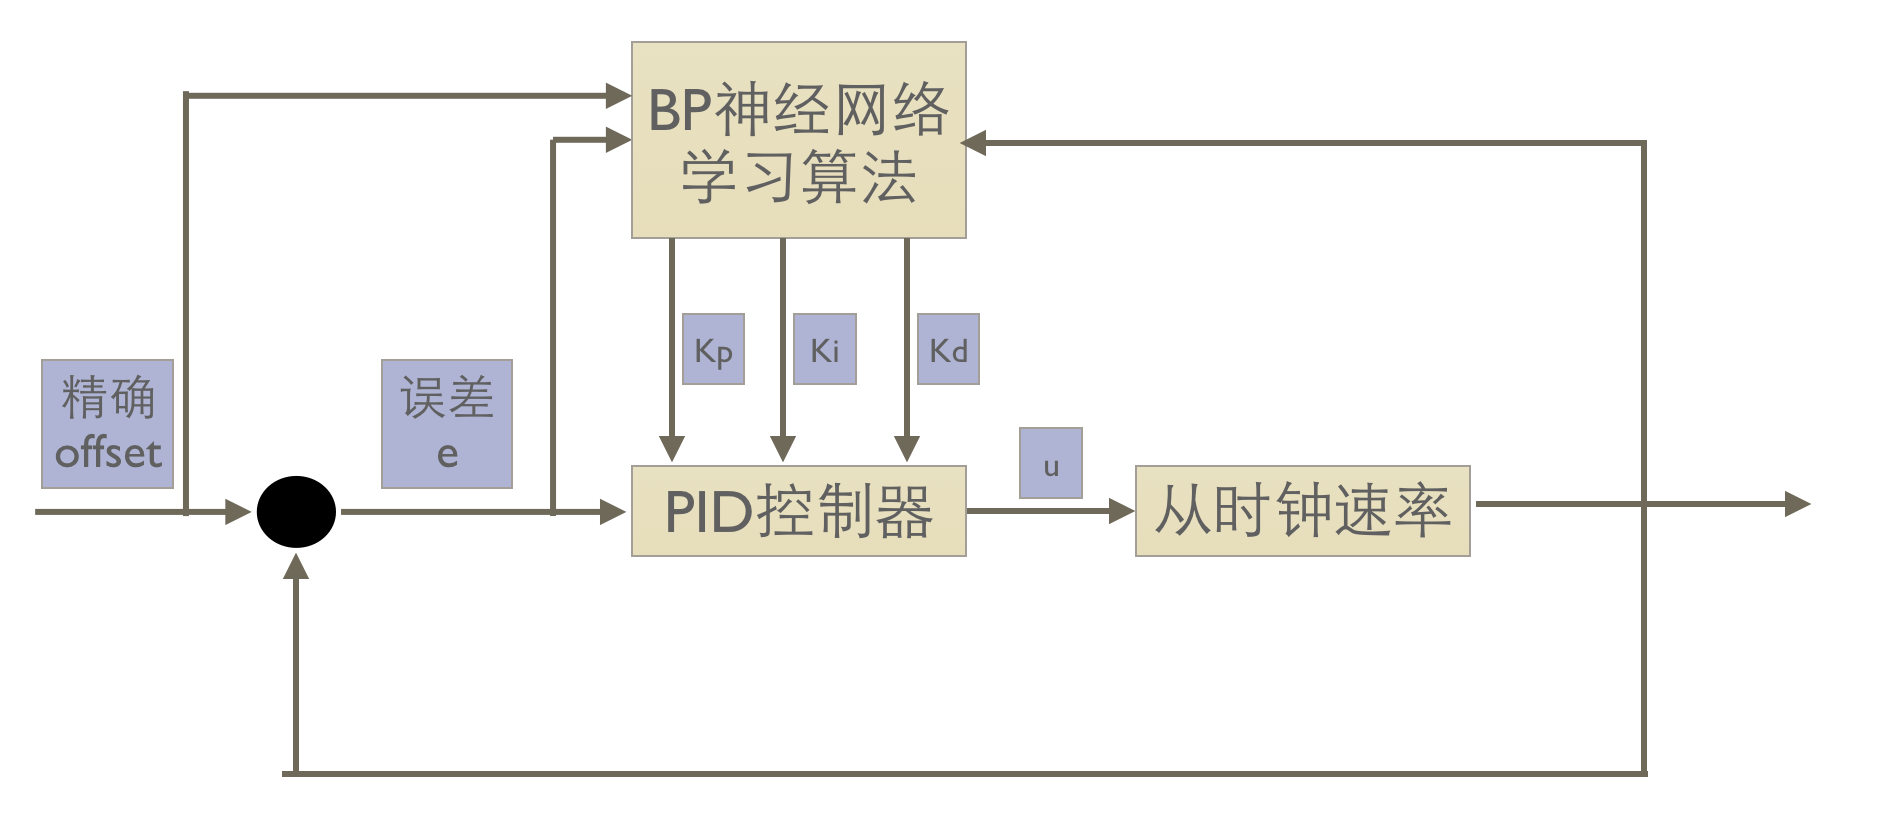
\includegraphics[width=10cm]{bp_neural_network_PID}
    \bicaption[fig:bp_neural_network_PID]{基于BP神经网络的PID控制系统结构图}{基于BP神经网络的PID控制系统结构图}{Fig}{The structure combining BP neural network with PID controller}
  \end{minipage}     
\end{figure}

\subsection{BP神经网络结构}
下图\ref{fig:bp_neural_network}为BP\footnote{Back Propagation 误差反向传播}神经网络结构图,从左往右依次为输入层、隐含层、输出层,下文将依据该结构,将伺服系统分成前向传播过程和误差反向传播过程来分别讲述。
\begin{figure}[!hbp]
  \centering
  \begin{minipage}[b]{0.6\textwidth}
    \captionstyle{\centering}
    \centering
    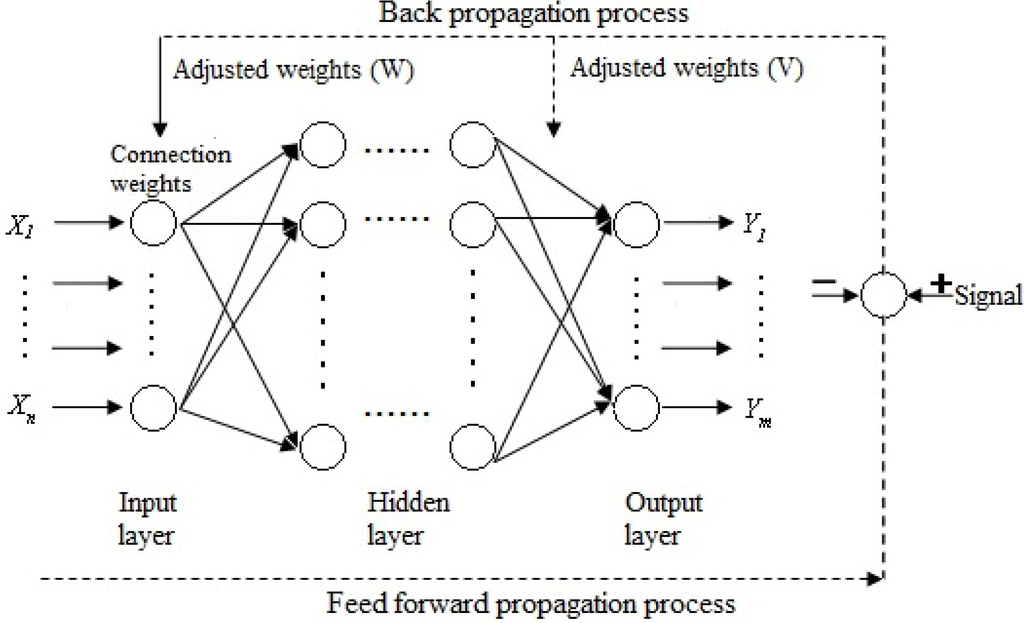
\includegraphics[width=10cm]{BP_neural_network}
    \bicaption[fig:bp_neural_network]{BP神经网络结构图}{BP神经网络结构图}{Fig}{The structure of BP neural network}
  \end{minipage}     
\end{figure}

\subsection{前向计算过程}
该过程是指输入变量依次经过输入层、隐含层直到输出层的过程。首先,对于输入层,我们可以选取k个主从偏差样本作为神经网络的输入。该样本个数k若太大,则会导致训练时间过长,系统需要较长时间的收敛过程;反之,若样本个数$K_{i}$太小,则会导致达不到学习效果\supercite{69}。在此,本人将$K_{i}$选取为4。所以,输入层的输入为:
\begin{align}
	input_{1} = offset_{c}, input_{2} = offset_{(c-1)}, \\
	input_{3} = offset_{(c-2)}, input_{4} = offset_{(c-3)}, 
\end{align}
其中,$offset_{c}$是表示当前时刻计算得到的时延值。所以,在输入层第i个输入节点的输出值为:
\begin{align}
	InputLayer\_Output_{i} = input_{i} \qquad i = 1, 2, 3, 4
\end{align}

然后,在隐含层有$K_{h}$个神经元节点,那么假设对于隐含层的第j个神经元的输入为:
\begin{align}
	HiddenLayer\_Input_{j} = \sum_{j=1}^{K_{h}}(W_{ij}InputLayer\_Output_{i})
\end{align}
即每一个隐含层节点的输入为所有输入层节点输出值乘以权值的总和。我们可以得到其隐含层节点的输出值为:
\begin{align}
	HiddenLayer\_Output_{j} = f(HiddenLayer\_Input_{j}) \qquad j = 1, 2 \cdots K_{h}
\end{align}

最后,在输出层,我们只选取三个输出节点,这三个节点分别对外提供三个控制参数$K_{i}$、$K_{p}$、$K_{d}$。
\begin{align}
K_{o} = 3
\end{align}
对于其中第z个输出节点,可以得到其输入值为:
\begin{align}
OutputLayer\_Input_{z} = \sum_{j=1}^{K_{h}}(W_{jz}HiddenLayer\_Output_{j}) \qquad z = 1, 2, 3
\end{align}
同时,我们可以得到第z个输出节点的最终输出值为:
\begin{align}
OutputLayer\_Output_{z} = g(HiddenLayer\_Input_{j}) \qquad j = 1, 2 \cdots K_{o}
\end{align}
其中,我们依次取各个输出为如下对应控制参数:
\begin{align}
K_{p} = OutputLayer\_Output_{1}
K_{i} = OutputLayer\_Output_{2}
K_{d} = OutputLayer\_Output_{3}
\end{align}

在上面的几个方程中,我们用$W_{ij}$来表示输入层到隐含层加权系数,然后用$W_{jz}$来表示隐含层到输出层的加权系数。另外,对于活化函数有多种选择方式,本人对于输入层\-隐含层及隐含层\-输出层分别取下面两个活化函数:
\begin{align}
Log-Sigmoid : f(x) = \frac{1}{1 + e^{-x}} \\
Sigmoid : g(x) = \frac{e^{x} - e^{-x}}{e^{x} + e^{-x}}
\end{align}

至此,我们已经可以从输出层得到三个控制参数$K_{i}$、$K_{p}$、$K_{d}$。但是,目前得到的三个控制参数并不能保证系统稳定,我们还需要误差反向传播过程,将实际误差反向传回给神经网络,并依靠该误差来进行加权系数的校正。

\subsection{误差反向传播}
根据上文中,我们已经了解到了BP神经网络算法中的固有缺陷,同时本人已经在上文中介绍响应的改进算法,下面,我们就该增加动量法来进行反向传播调节的实际。

首先,我们依据最速下降法取性能指标函数为:
\begin{align}
T(k) = \frac{1}{2}(Rin(k) - Yout(k))^{2}
\end{align}
同时,我们利用近似最速下降法来更新该系统中的各个权值,具体的更新方法如下:
\begin{align}
\Delta W_{jz}(k) = -\eta \frac{\partial E(k)}{\partial W_{jz}} + \alpha \Delta W_{jz}(k-1)
\end{align}
在上式子中,$\alpha$用来表示惯性系数,$\eta$用来表示学习速度,式子的后半部分是指在k-1时刻网络权值的修改方向,这也正是上文中所介绍的增加动量法的权值更新方式。也就是说,如果第k次的更新方向与k-1次相同,那么后半部分就为正,从而加速整个更新过程,相反,如果二者方向不同,那么后半部分为负,从而起到稳定更新算法的作用。

\section{基于离线BP神经网络的PID控制策略小结}
利用上述基于BP神经网络的PID控制器,通过神经网络与输入样本值来计算控制器所需的三个控制参数,从而实现对从时钟的校正。在下文中,我们会对这种方法的效果进行仿真,结合该结果我们可以看出,采用离线神经网络训练后的PID控制器可以起到不错的优化效果,在一定程度上能提高时钟伺服系统的稳定性和适应性。

但是,我们也能发现其中仍然存在的缺陷。一般而言神经网络需要一定的训练时间,对于资源非常有限的交换机设备而言,在线进行神经网络训练目前而言是不够现实的。所以,我们只能采用离线训练的方法,来降低该方法对交换机本身的负载压力。因此,这势必会导致神经网络的实时性有所缺陷,即不能实时利用采集样本数据来进行训练。

综上所述,离线BP神经网络由于其能采用实际的时延样本来进行训练,所以能够取得不错的鲁棒性和自适应性。这是其他方法,例如常规PI控制策略所不具备的,它所能带来的高稳定性和高鲁棒性也是对高精度时钟同步系统而言非常需要的。但是,我们也应该明确这种方法存在的固有漏洞,那就是神经网络方法本身会需要较多的计算资源和空间资源,才能取得良好的效果。根据当前的应用实践,本人认为离线BP神经网络是目前而言具备良好的应用价值的。未来随着交换机等设备的升级和对时钟精度的更高要求,或许有可能在上面使用在线BP神经网络来进一步改善鲁棒性和自适应性。







